\documentclass{standalone}
\usepackage{tikz}
\usepackage{xcolor}
\usetikzlibrary{patterns, positioning}
\usetikzlibrary{shapes.misc}
\usepackage[outline]{contour}
\contourlength{1.5pt} 


\begin{document}
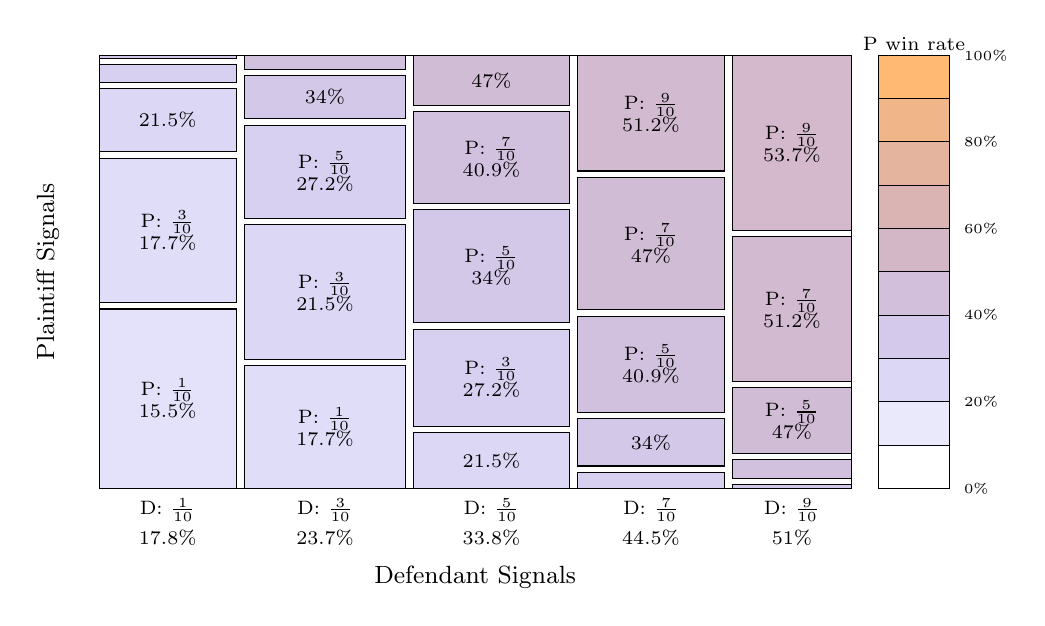
\begin{tikzpicture}
\newcommand{\DFractionOffset}{0.4}
\newcommand{\AxisLabelYAdjust}{-0.235}
\draw[draw=black] (0.6,2) rectangle (10.15,7.5);
\draw[fill=blue!85!orange!15!white!83!white, draw=black] (0.6,2) rectangle (2.3412,4.278);
\draw (1.4706035369571255, 3.139020128248707) node[font=\scriptsize, text=black, align=center] {P: $\frac{1}{10}$\\ 15.5\%};
\draw[fill=blue!82!orange!18!white!82!white, draw=black] (0.6,4.358) rectangle (2.3412,6.1935);
\draw (1.4706035369571255, 5.275763857768809) node[font=\scriptsize, text=black, align=center] {P: $\frac{3}{10}$\\ 17.7\%};
\draw[fill=blue!78!orange!22!white!81!white, draw=black] (0.6,6.2735) rectangle (2.3412,7.0792);
\draw (1.4706035369571255, 6.676326768134136) node[font=\scriptsize, text=black, align=center] {21.5\%};
\draw[fill=blue!73!orange!27!white!79!white, draw=black] (0.6,7.1592) rectangle (2.3412,7.3794);
\draw[fill=blue!66!orange!34!white!77!white, draw=black] (0.6,7.4594) rectangle (2.3412,7.5);
\draw (1.4706035369571255, 1.6) node[anchor=north, font=\scriptsize, text=black] {17.8\%};
\draw (1.4706035369571255, {1.6 + \DFractionOffset}) node[anchor=north, font=\scriptsize, text=black] {D: $\frac{1}{10}$};
\draw[fill=blue!82!orange!18!white!82!white, draw=black] (2.4412,2) rectangle (4.4962,3.5552);
\draw (3.4687052538644796, 2.7775910739370935) node[font=\scriptsize, text=black, align=center] {P: $\frac{1}{10}$\\ 17.7\%};
\draw[fill=blue!78!orange!22!white!81!white, draw=black] (2.4412,3.6352) rectangle (4.4962,5.3516);
\draw (3.4687052538644796, 4.493387754188655) node[font=\scriptsize, text=black, align=center] {P: $\frac{3}{10}$\\ 21.5\%};
\draw[fill=blue!73!orange!27!white!79!white, draw=black] (2.4412,5.4316) rectangle (4.4962,6.6139);
\draw (3.4687052538644796, 6.022762654552329) node[font=\scriptsize, text=black, align=center] {P: $\frac{5}{10}$\\ 27.2\%};
\draw[fill=blue!66!orange!34!white!77!white, draw=black] (2.4412,6.6939) rectangle (4.4962,7.244);
\draw (3.4687052538644796, 6.968951150765405) node[font=\scriptsize, text=black, align=center] {34\%};
\draw[fill=blue!59!orange!41!white!75!white, draw=black] (2.4412,7.324) rectangle (4.4962,7.5);
\draw (3.4687052538644796, 1.6) node[anchor=north, font=\scriptsize, text=black] {23.7\%};
\draw (3.4687052538644796, {1.6 + \DFractionOffset}) node[anchor=north, font=\scriptsize, text=black] {D: $\frac{3}{10}$};
\draw[fill=blue!78!orange!22!white!81!white, draw=black] (4.5962,2) rectangle (6.5698,2.7108);
\draw (5.582985063146499, 2.355411285433061) node[font=\scriptsize, text=black, align=center] {21.5\%};
\draw[fill=blue!73!orange!27!white!79!white, draw=black] (4.5962,2.7908) rectangle (6.5698,4.0219);
\draw (5.582985063146499, 3.406384672573817) node[font=\scriptsize, text=black, align=center] {P: $\frac{3}{10}$\\ 27.2\%};
\draw[fill=blue!66!orange!34!white!77!white, draw=black] (4.5962,4.1019) rectangle (6.5698,5.5423);
\draw (5.582985063146499, 4.822141884528729) node[font=\scriptsize, text=black, align=center] {P: $\frac{5}{10}$\\ 34\%};
\draw[fill=blue!59!orange!41!white!75!white, draw=black] (4.5962,5.6223) rectangle (6.5698,6.7834);
\draw (5.582985063146499, 6.2028912721116845) node[font=\scriptsize, text=black, align=center] {P: $\frac{7}{10}$\\ 40.9\%};
\draw[fill=blue!53!orange!47!white!73!white, draw=black] (4.5962,6.8634) rectangle (6.5698,7.5);
\draw (5.582985063146499, 7.1817227747237125) node[font=\scriptsize, text=black, align=center] {47\%};
\draw (5.582985063146499, 1.6) node[anchor=north, font=\scriptsize, text=black] {33.8\%};
\draw (5.582985063146499, {1.6 + \DFractionOffset}) node[anchor=north, font=\scriptsize, text=black] {D: $\frac{5}{10}$};
\draw[fill=blue!73!orange!27!white!79!white, draw=black] (6.6698,2) rectangle (8.5463,2.2044);
\draw[fill=blue!66!orange!34!white!77!white, draw=black] (6.6698,2.2844) rectangle (8.5463,2.8868);
\draw (7.608018511371177, 2.5855713093234307) node[font=\scriptsize, text=black, align=center] {34\%};
\draw[fill=blue!59!orange!41!white!75!white, draw=black] (6.6698,2.9668) rectangle (8.5463,4.1879);
\draw (7.608018511371177, 3.577332958119449) node[font=\scriptsize, text=black, align=center] {P: $\frac{5}{10}$\\ 40.9\%};
\draw[fill=blue!53!orange!47!white!73!white, draw=black] (6.6698,4.2679) rectangle (8.5463,5.9512);
\draw (7.608018511371177, 5.109563637945241) node[font=\scriptsize, text=black, align=center] {P: $\frac{7}{10}$\\ 47\%};
\draw[fill=blue!49!orange!51!white!71!white, draw=black] (6.6698,6.0312) rectangle (8.5463,7.5);
\draw (7.608018511371177, 6.765605826553816) node[font=\scriptsize, text=black, align=center] {P: $\frac{9}{10}$\\ 51.2\%};
\draw (7.608018511371177, 1.6) node[anchor=north, font=\scriptsize, text=black] {44.5\%};
\draw (7.608018511371177, {1.6 + \DFractionOffset}) node[anchor=north, font=\scriptsize, text=black] {D: $\frac{7}{10}$};
\draw[fill=blue!66!orange!34!white!77!white, draw=black] (8.6463,2) rectangle (10.15,2.047);
\draw[fill=blue!59!orange!41!white!75!white, draw=black] (8.6463,2.127) rectangle (10.15,2.3675);
\draw[fill=blue!53!orange!47!white!73!white, draw=black] (8.6463,2.4475) rectangle (10.15,3.283);
\draw (9.398135165132032, 2.8652487377714904) node[font=\scriptsize, text=black, align=center] {P: $\frac{5}{10}$\\ 47\%};
\draw[fill=blue!49!orange!51!white!71!white, draw=black] (8.6463,3.363) rectangle (10.15,5.1959);
\draw (9.398135165132032, 4.279420441830121) node[font=\scriptsize, text=black, align=center] {P: $\frac{7}{10}$\\ 51.2\%};
\draw[fill=blue!46!orange!54!white!70!white, draw=black] (8.6463,5.2759) rectangle (10.15,7.5);
\draw (9.398135165132032, 6.387935314752054) node[font=\scriptsize, text=black, align=center] {P: $\frac{9}{10}$\\ 53.7\%};
\draw (9.398135165132032, 1.6) node[anchor=north, font=\scriptsize, text=black] {51\%};
\draw (9.398135165132032, {1.6 + \DFractionOffset}) node[anchor=north, font=\scriptsize, text=black] {D: $\frac{9}{10}$};
\node[font=\small, text=black] at (5.375, {1.1 + \AxisLabelYAdjust}) {Defendant Signals};
\node[font=\small, text=black, rotate=90] at (-0.050000000000000044, 4.75) {Plaintiff Signals};
\draw[draw=black] (10.5,2) rectangle (11.4,7.5);
\draw (10.95, 7.65) node[font=\scriptsize, text=black] {P win rate};
\draw[fill=blue!100!orange!0!white!88!white, draw=black] (10.5,2) rectangle (11.4,2.55);
\draw[fill=blue!89!orange!11!white!84!white, draw=black] (10.5,2.55) rectangle (11.4,3.1);
\draw[fill=blue!78!orange!22!white!81!white, draw=black] (10.5,3.1) rectangle (11.4,3.65);
\draw[fill=blue!67!orange!33!white!77!white, draw=black] (10.5,3.65) rectangle (11.4,4.2);
\draw[fill=blue!56!orange!44!white!73!white, draw=black] (10.5,4.2) rectangle (11.4,4.75);
\draw[fill=blue!44!orange!56!white!70!white, draw=black] (10.5,4.75) rectangle (11.4,5.3);
\draw[fill=blue!33!orange!67!white!66!white, draw=black] (10.5,5.3) rectangle (11.4,5.85);
\draw[fill=blue!22!orange!78!white!62!white, draw=black] (10.5,5.85) rectangle (11.4,6.4);
\draw[fill=blue!11!orange!89!white!59!white, draw=black] (10.5,6.4) rectangle (11.4,6.95);
\draw[fill=blue!0!orange!100!white!55!white, draw=black] (10.5,6.95) rectangle (11.4,7.5);
\draw (11.46, 2) node[anchor=west, font=\tiny, text=black] {0\%};
\draw (11.46, 3.1) node[anchor=west, font=\tiny, text=black] {20\%};
\draw (11.46, 4.2) node[anchor=west, font=\tiny, text=black] {40\%};
\draw (11.46, 5.3) node[anchor=west, font=\tiny, text=black] {60\%};
\draw (11.46, 6.4) node[anchor=west, font=\tiny, text=black] {80\%};
\draw (11.46, 7.5) node[anchor=west, font=\tiny, text=black] {100\%};


\end{tikzpicture}
\end{document}